\chapter{Capítulo Z}
\label{cap:capZ}
	
	Citando \cite{Coope1977}.
	
	\begin{figure}[htbp]
		\centering
			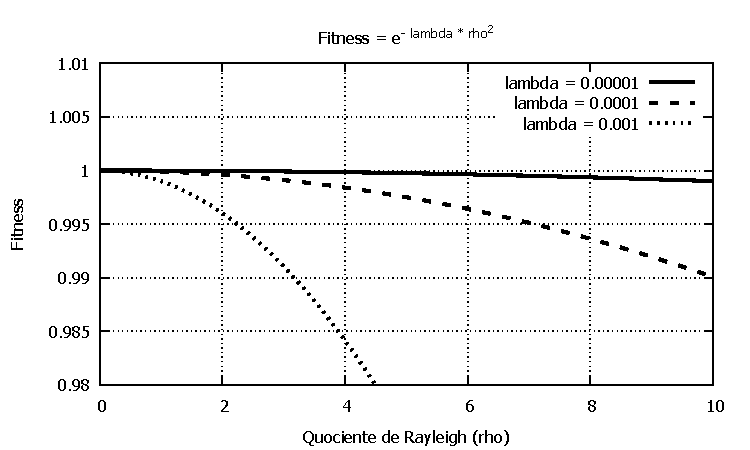
\includegraphics{figs/varios-fit-mono-zoom.pdf}
		\caption{Zoom próximo do pico}
		\label{fig:varios-fit-mono-zoom}
	\end{figure}
	
		
	$$
		\frac{df}{d\rho} = -2\lambda(\rho - \rho0)e^{-\lambda(\rho - \rho0)^2}
	$$
	
		
	\begin{figure}[htbp]
		\centering
			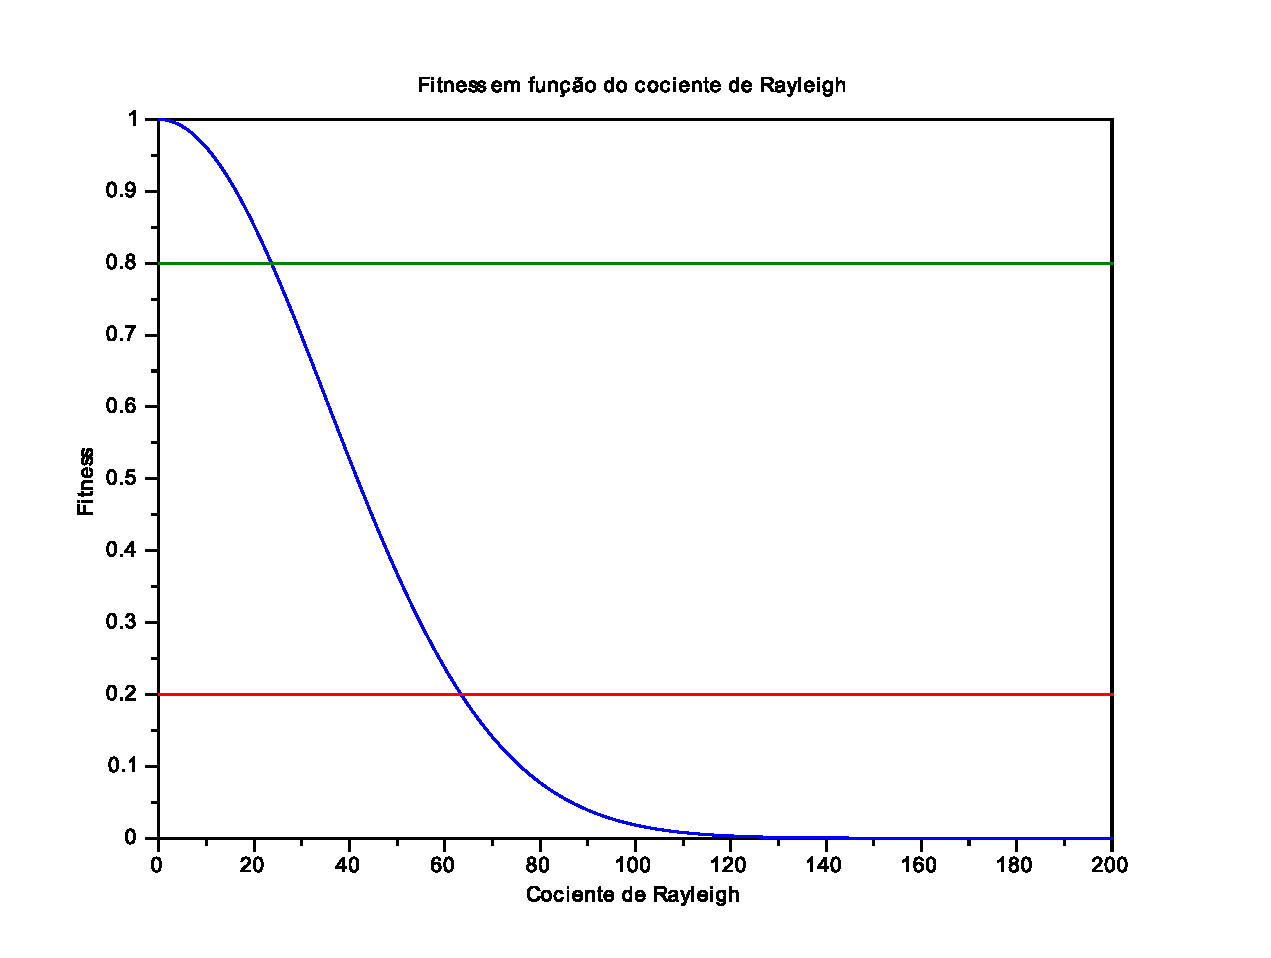
\includegraphics[width=0.90\textwidth]{figs/resultados/fitness_boaRegiao.pdf}
		\caption{Boa região para o fitness (entre as duas linhas)}
		\label{fig:fitness_boaRegiao}
	\end{figure}
	
	
	% Table generated by Excel2LaTeX from sheet 'Plan2'
\begin{tabular}{rr}

       \textit{rho} &          \textit{f} \\

      -0,1 &   0,999996 \\

     -0,09 &   0,999997 \\

     -0,08 &   0,999997 \\

     -0,07 &   0,999998 \\

     -0,06 &   0,999999 \\

     -0,05 &   0,999999 \\

     -0,04 &   0,999999 \\

     -0,03 &          1 \\

     -0,02 &          1 \\

     -0,01 &          1 \\

         0 &          1 \\

      0,01 &          1 \\

      0,02 &          1 \\

      0,03 &          1 \\

      0,04 &   0,999999 \\

      0,05 &   0,999999 \\

      0,06 &   0,999999 \\

      0,07 &   0,999998 \\

      0,08 &   0,999997 \\

      0,09 &   0,999997 \\

       0,1 &   0,999996 \\

\end{tabular}  
		
	
	\begin{figure}[pt]
	\centering
		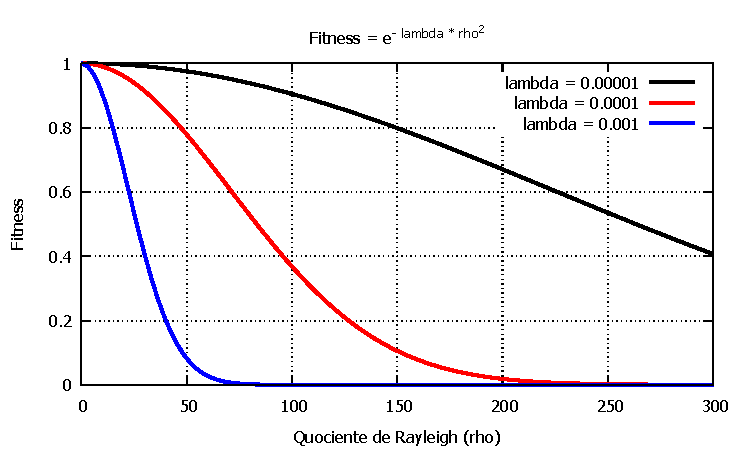
\includegraphics{figs/varios-fits-color.pdf}
	\caption{Fitness em função do lambda $-$ colorido}
	\label{fig:varios-fits-color}
\end{figure}

\begin{figure}[pb]
	\centering
		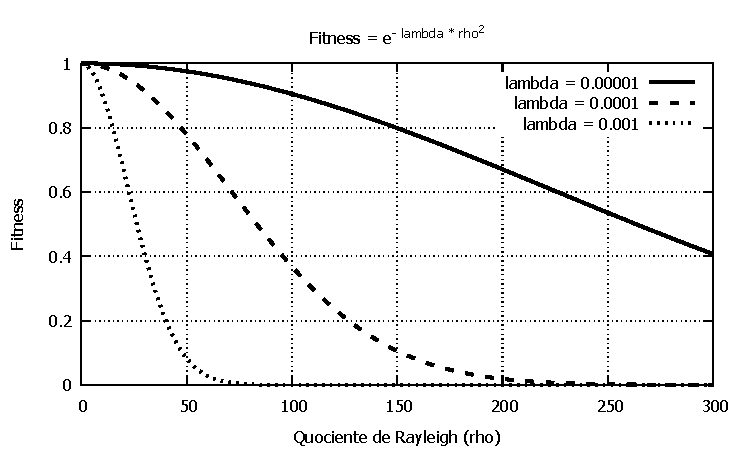
\includegraphics{figs/varios-fits-mono.pdf}
	\caption{Fitness em função do lambda}
	\label{fig:varios-fits-mono}
\end{figure}